\section{Motivations}

Volumetric Displays are a new and exciting technology that has the potential to revolutionize the way we interact with computers. They are a type of 3D display that can be viewed from any angle without the need for special glasses by multiple people simultaneously. \cite{1492264} These displays differ from a virtual reality experience in that they are not immersive, but rather they are a window into a virtual world (See Fig~\ref{fig:volumetric-display-examples}). There is no consensus on what the best way to build a volumetric display is and as we cover in the background section many approaches are being attempted by research groups both academic and industrial.

% \begin{figureBox}[label={fig:volumetric-display-examples}]{Two different volumetric displays}
%   \begin{minipage}[c]{0.48\textwidth}
%     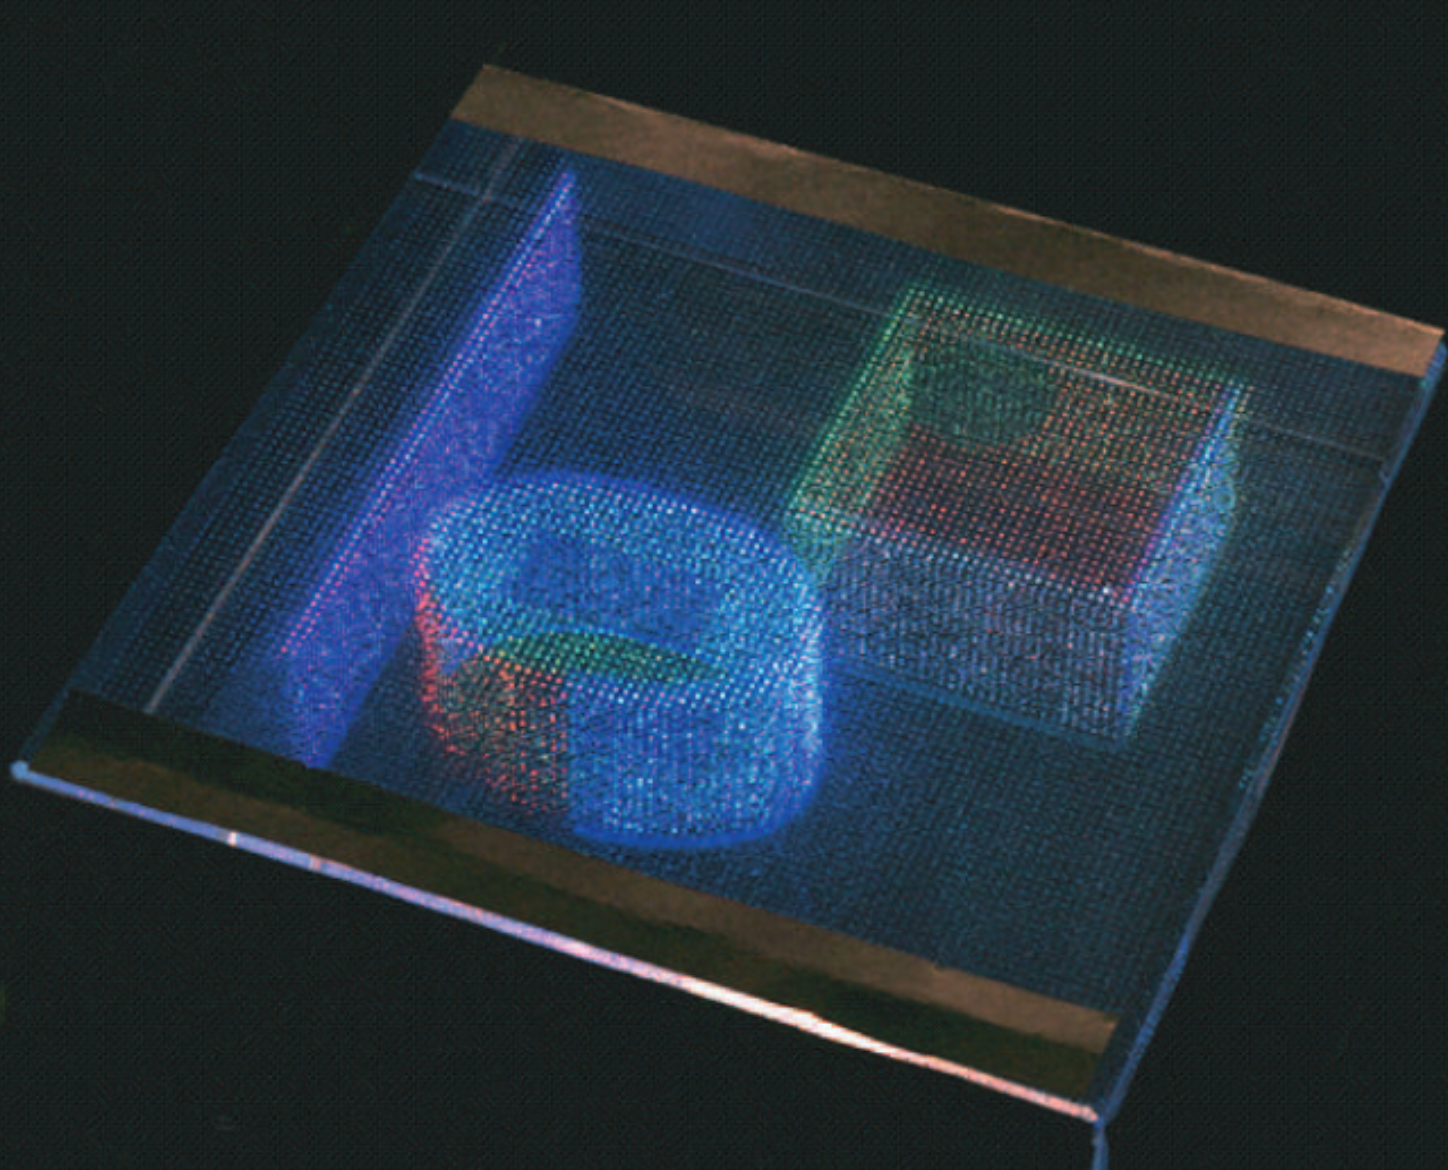
\includegraphics[width = \linewidth, keepaspectratio]{./introduction/figures/passive optical scatterers.png} \\
%     \small {a) A volumetric display created at Columbia University using passive optical scattering \cite{10.1145/1179849.1179982}.}
%   \end{minipage}\hfill
%   \begin{minipage}[c]{0.48\textwidth}
%     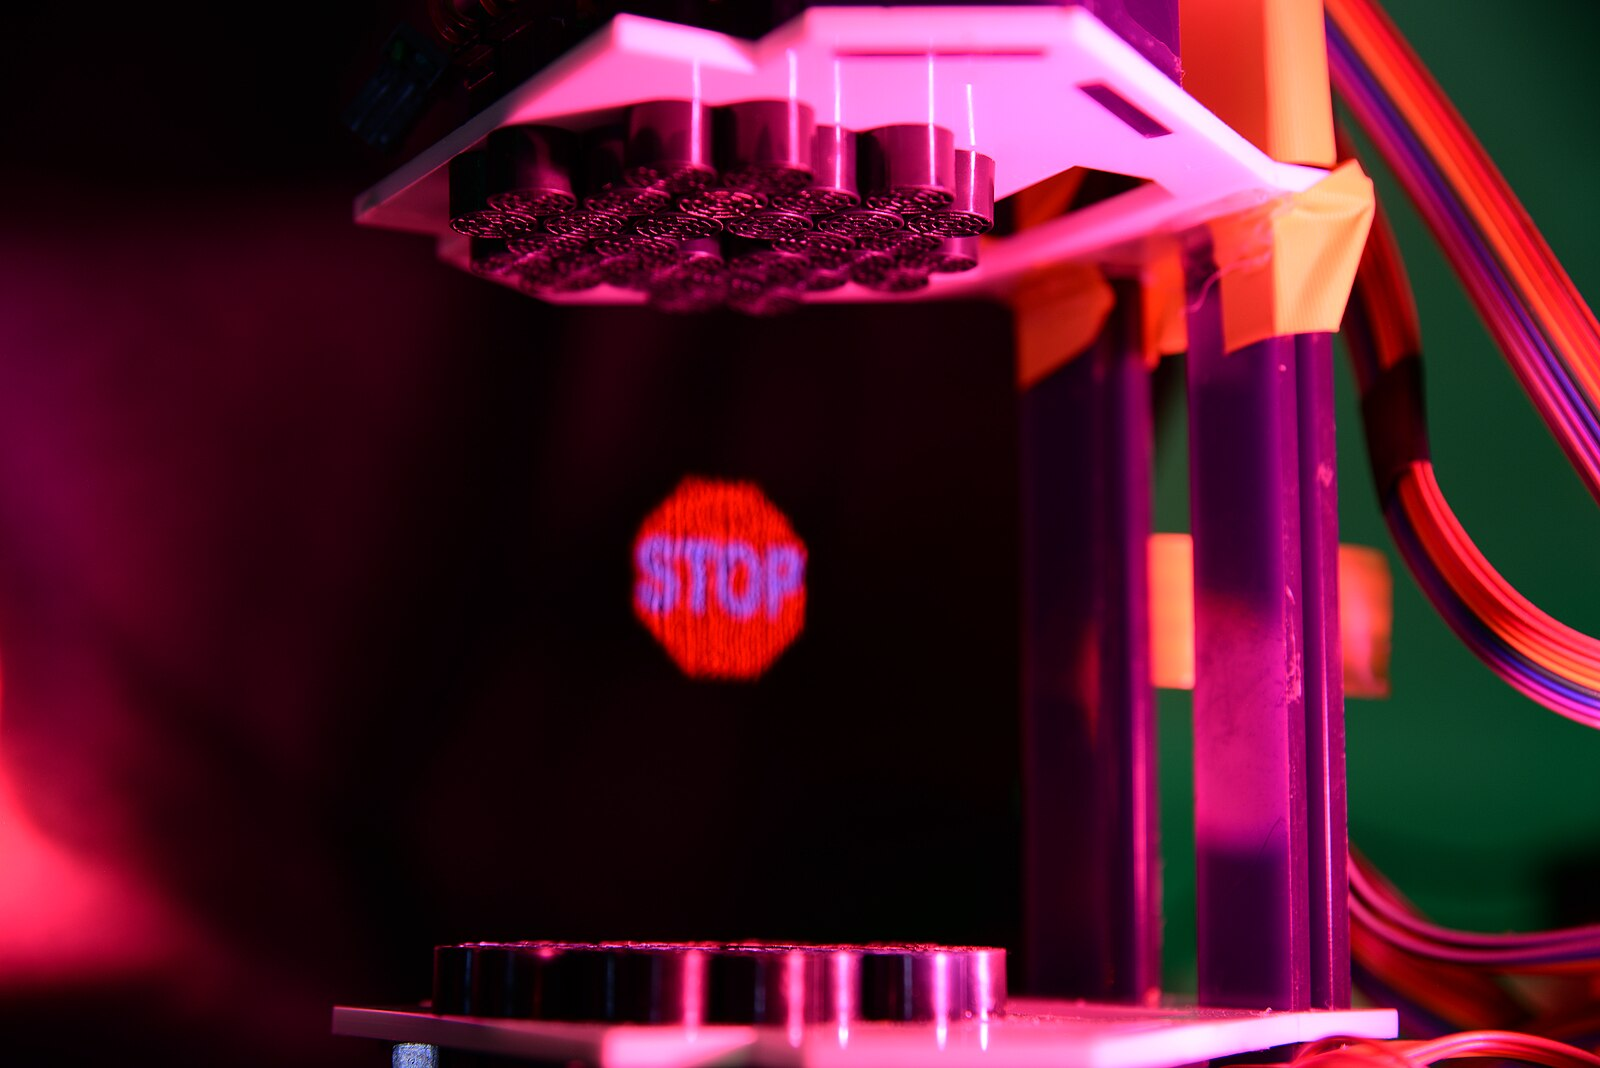
\includegraphics[width = \linewidth, keepaspectratio]{./introduction/figures/acoustophoretic display.jpg} \\
%     \small {b) A volumetric display created at Bristol University using acoustic trapping \cite{10.1063/1.5113467}}
%   \end{minipage}
% \end{figureBox}
\begin{tcbraster}[raster columns=2,raster equal height=rows]
\pictureBox{a) A volumetric display created at Columbia University using passive optical scattering \cite{10.1145/1179849.1179982}}{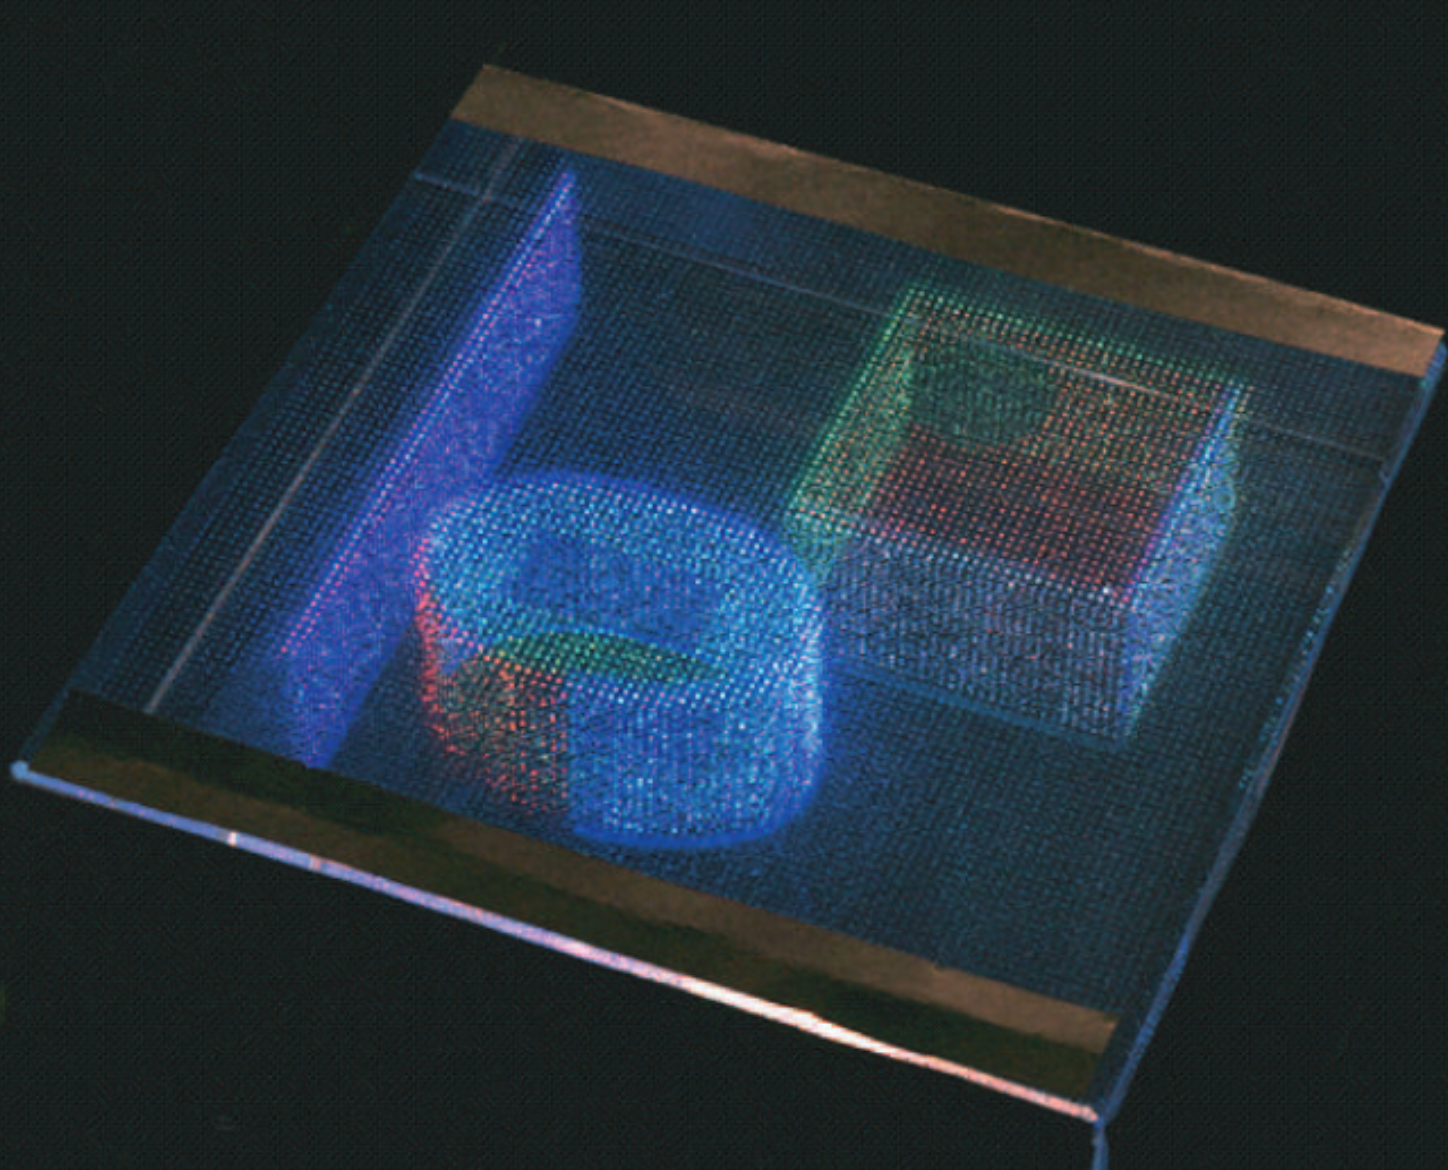
\includegraphics[width = \linewidth, keepaspectratio]{./introduction/figures/passive optical scatterers.png}}
\hfill
\pictureBox{b) A volumetric display created at Bristol University using acoustic trapping \cite{10.1063/1.5113467}}{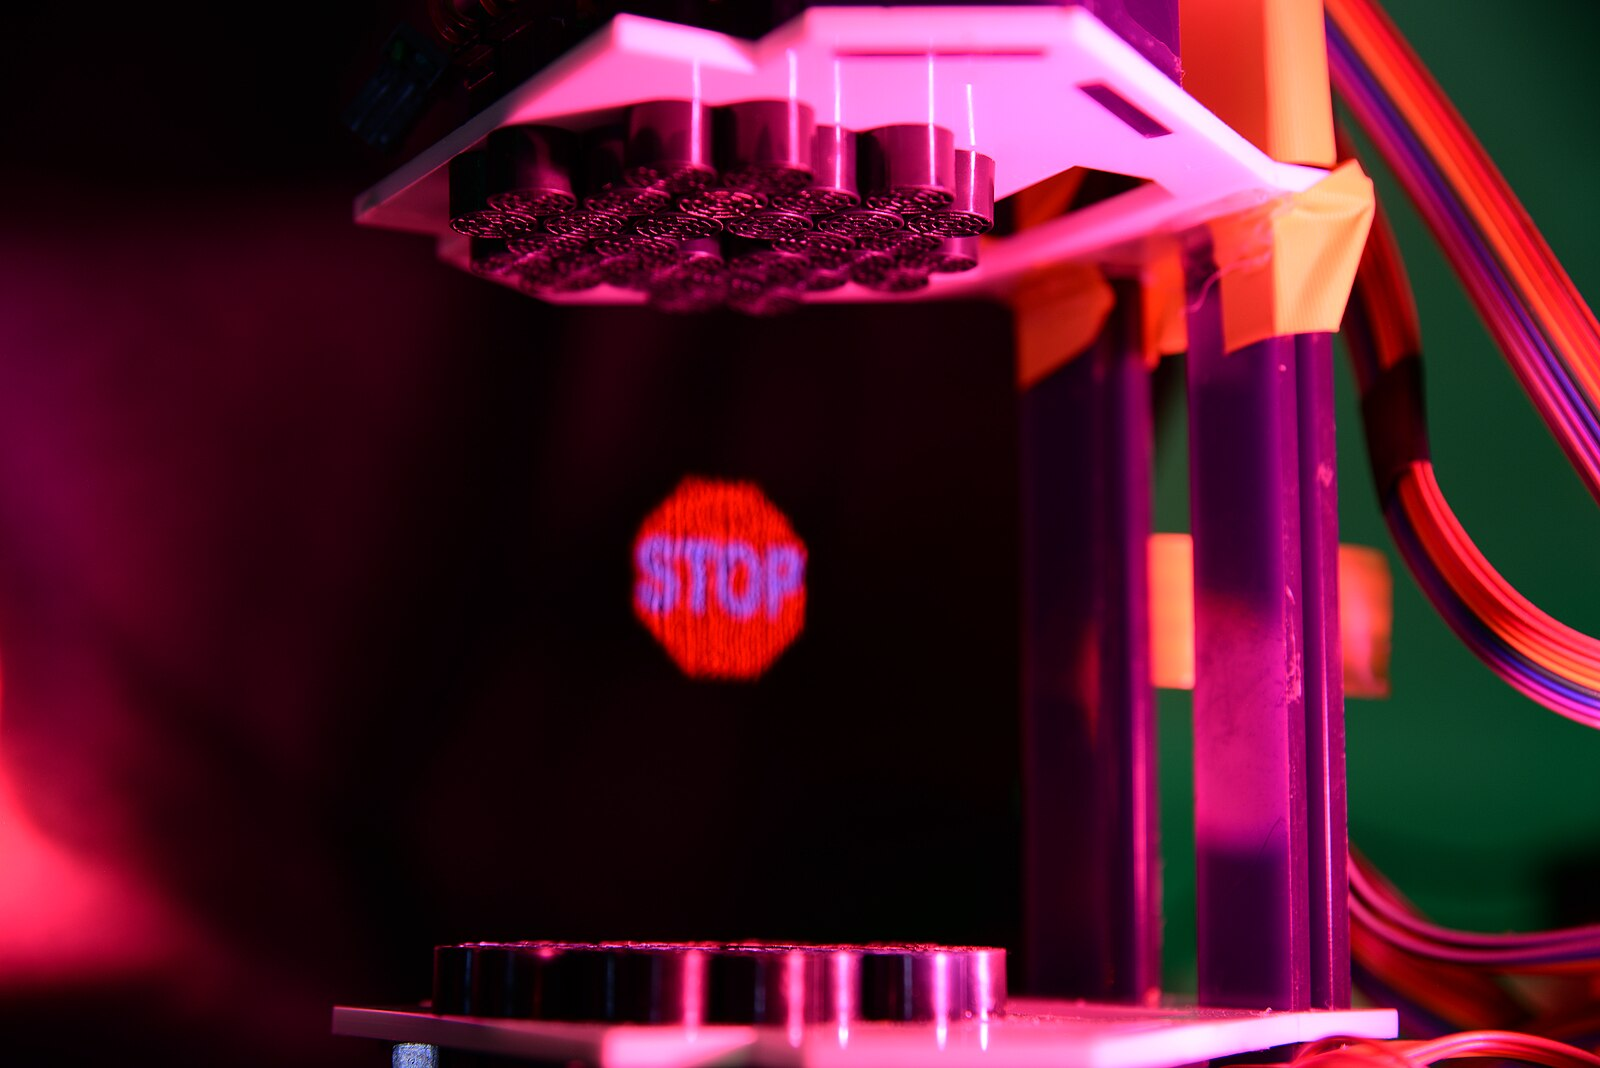
\includegraphics[width = \linewidth, keepaspectratio]{./introduction/figures/acoustophoretic display.jpg}}
\end{tcbraster}

It is difficult to conduct human-computer interaction (HCI) research into volumetric displays because these devices are not widely available, expensive to manufacture, and have high bandwidth requirements. This makes it difficult to conduct user studies and experiments. People have created virtual simulations of volumetric displays to try and solve this problem (see background), but these solutions are often complicated and expensive to replicate.

\section{Objectives}

With this project, we aim to provide a cheap, multi-platform, lightweight and simple platform for simulating volumetric displays. We hope that this will enable researchers to conduct HCI research into volumetric displays without the need for expensive hardware. We aim to make the following contributions:
\subsection{Volumetric Simulator}
We plan to create a platform for simulating volumetric displays that is:
\begin{itemize}
  \item \textbf{Multi-platform}: We package our platform in the nix package manager \cite{dolstra2004nix} which allows it to be easily run on any platform and hardware that supports nix by running a single line of code \texttt{sudo nix run github:RobbieBuxton/VolumetricSim}.

  \item \textbf{Lightweight}: By using simple rending algorithms in OpenGL \cite{rost2009opengl} to render a volumetric display our software is computationally cheap to run compared to rendering/games engines that might be used typically for HCI research like Unity.

  \item \textbf{Cheap}: By relying on only a depth camera and standard monitor our software requires minimal hardware to run, making research conducted on our platform cheaper and easy to run.

  \item \textbf{Simple}: We have designed our software to be as simple as possible by taking advantage of the nix package manager to handle all the dependencies and by depending on external libraries like \texttt{dlib} \cite{10.5555/1577069.1755843} to handle more complicated tasks like face detection. This makes it easy to replicate and modify.

  \item \textbf{Reproducible:} By building with nix we can guarantee that any experiments conducted using the simulator will be completely reproducible. (See background)
\end{itemize}

\subsection{User experiment}
We plan to conduct an HCI user study to demonstrate the utility of our volumetric simulation platform. We will conduct a user study to compare the effectiveness of using hand tracking to interact directly with an ethereal/incorporeal volumetric display compared to a via teleoperation with a corporeal/tangible display (See evaluation).
